\section{Ход работы}
\subsection{Знакомство с экспериментальной установкой}

Перед началом работы было проведено ознакомление с установкой для получания крутильных колебаний. Проволока натянуна безупречно. Рамка закреплена на ней жесточайшим образом. Устройство для возбуждения крутильных колебаний работает без нареканий. Колебания в вертикальной плоскости, к счастью, не возникают.

\subsection{Закрепление тела в рамке}

На данном этапе лабораторной работы был осуществлен процесс закрепления тел в рамке с использованием специальных углублений на телах и винтов, находящихся на рамке. 

Процесс закрепления тел в рамке был внимательно выполнен в соответствии с предоставленными инструкциями, тем самым мы обеспечили надежность и стабильность закрепленных тел в экспериментальной установке.

\subsection{Определение амплитуды крутильных колебаний}

Перед каждой серией измерений, включая пустую рамку или рамку с предварительным закреплением тела, произведено важное действие — выбор оптимальной амплитуды крутильных колебаний. Этот процесс характеризуется следующими этапами:

\begin{enumerate}
    \item Проведение измерения периода колебаний, определяемого по 10-15 колебаниям рамки.
    \item Уменьшение амплитуды в два раза, согласно установленным критериям. Оцененка изменения периода колебаний при уменьшении амплитуды.
    \item В случае изменения периода колебаний после уменьшения амплитуды, произведение коррекции амплитуды в соответствии с установленными критериями.
    \end{enumerate}

    Примечание: процесс коррекции повторяется до тех пор, пока не будет достигнута оптимальная амплитуда, при которой период колебаний остается постоянным.

Этот этап эксперимента направлен на обеспечение точности и надежности измерений путем правильного выбора амплитуды крутильных колебаний перед каждой серией наблюдений.

\subsection{Измерение периодов колебаний для пустой рамки и тел в различных положениях}

На данном этапе исследования проведены измерения периодов колебаний для как пустой рамки, так и тел, находящихся в различных положениях относительно оси колебаний. Процедура измерения включала в себя следующие этапы:

\begin{enumerate}
\item Пустая рамка.

\begin{itemize}
    \item Проведено измерение периода колебаний для пустой рамки, при этом осуществлены не менее трех повторных измерений для обеспечения достоверности данных.
Каждое измерение включало в себя фиксацию времени, затраченного на 10-15 колебаний.
\end{itemize}


    \item Тела в различных положениях.

    \begin{itemize}
        \item Каждое тело было размещено в рамке в различных положениях относительно оси колебаний.
\item Для каждого положения тела были проведены измерения периода колебаний, повторенные от трех до пяти раз. Результаты измерений приведены в таблицах \ref{tabl1}, \ref{tabl2}, \ref{tabl3}.
\item Зафиксированы временные интервалы, необходимые для осуществления 10-15 колебаний для каждого положения тела.
    \end{itemize}


\item Обработка данных.

Для каждого измерения были рассчитаны средние значения периода колебаний по формуле:

    \begin{equation}
        T_\text{ср} = \frac{1}{N}\sum_{i=1}^{N}T_i,
    \end{equation}
    где $N$ -- количество измерений.

    Также была вычислена случайная погрешность измерений:
    \begin{equation}
        \sigma_\text{сл}=\sqrt{\frac{1}{N\left( N - 1 \right)}\sum_{i=1}^{N}\left( T_\text{ср} - T_i \right)^2 },
    \end{equation}
    
    и полная погрешность в пределах одной серии опытов: 
    \begin{equation}
    \sigma = \sqrt{\Delta_\text{с}^2+\sigma_\text{сл}^2}.
    \end{equation}

    В таблицу была записана полная относительная погрешность $\varepsilon_t^\text{полн}$ измерений среднего периода колебаний $T_\text{ср}$:

    \begin{equation}
        \varepsilon_t^\text{полн} = \frac{\sigma}{T_\text{ср}} 
    \end{equation}

    Из таблиц \ref{tabl2} и \ref{tabl3} видно, что периоды колебаний симметричных осей равны, а значит, параллелепипед действительно является симметричным.


\end{enumerate}

\newpage

\begin{table}[h!]
\centering
\begin{tabular}{|cccccc|}
\hline
\multicolumn{6}{|c|}{Только платформа} \\ \hline
\multicolumn{1}{|c|}{t,c} &
  \multicolumn{1}{c|}{N} &
  \multicolumn{1}{c|}{t,c} &
  \multicolumn{1}{c|}{$T_\text{ср}$} &
  \multicolumn{1}{c|}{$\sigma_t^\text{случ}$,c} &
  $\varepsilon_t^\text{полн},c$ \\ \hline
\multicolumn{1}{|c|}{45,15} &
  \multicolumn{1}{c|}{10} &
  \multicolumn{1}{c|}{4,515} &
  \multicolumn{1}{c|}{\multirow{5}{*}{4,515}} &
  \multicolumn{1}{c|}{\multirow{5}{*}{0,005}} &
  \multirow{5}{*}{0,009} \\ \cline{1-3}
\multicolumn{1}{|c|}{45,17} &
  \multicolumn{1}{c|}{10} &
  \multicolumn{1}{c|}{4,517} &
  \multicolumn{1}{c|}{} &
  \multicolumn{1}{c|}{} &
   \\ \cline{1-3}
\multicolumn{1}{|c|}{45,11} &
  \multicolumn{1}{c|}{10} &
  \multicolumn{1}{c|}{4,511} &
  \multicolumn{1}{c|}{} &
  \multicolumn{1}{c|}{} &
   \\ \cline{1-3}
\multicolumn{1}{|c|}{45,22} &
  \multicolumn{1}{c|}{10} &
  \multicolumn{1}{c|}{4,522} &
  \multicolumn{1}{c|}{} &
  \multicolumn{1}{c|}{} &
   \\ \cline{1-3}
\multicolumn{1}{|c|}{45,08} &
  \multicolumn{1}{c|}{10} &
  \multicolumn{1}{c|}{4,508} &
  \multicolumn{1}{c|}{} &
  \multicolumn{1}{c|}{} &
   \\ \hline
\multicolumn{6}{|c|}{Ось Z} \\ \hline
\multicolumn{1}{|c|}{t,c} &
  \multicolumn{1}{c|}{N} &
  \multicolumn{1}{c|}{t,c} &
  \multicolumn{1}{c|}{$T_\text{ср}$,c} &
  \multicolumn{1}{c|}{$\sigma_t^\text{случ}$,c} &
  $\varepsilon_t^\text{полн}$ \\ \hline
\multicolumn{1}{|c|}{56,22} &
  \multicolumn{1}{c|}{10} &
  \multicolumn{1}{c|}{5,622} &
  \multicolumn{1}{c|}{\multirow{5}{*}{5,633}} &
  \multicolumn{1}{c|}{\multirow{5}{*}{0,007}} &
  \multirow{5}{*}{0,007} \\ \cline{1-3}
\multicolumn{1}{|c|}{56,40} &
  \multicolumn{1}{c|}{10} &
  \multicolumn{1}{c|}{5,640} &
  \multicolumn{1}{c|}{} &
  \multicolumn{1}{c|}{} &
   \\ \cline{1-3}
\multicolumn{1}{|c|}{56,30} &
  \multicolumn{1}{c|}{10} &
  \multicolumn{1}{c|}{5,630} &
  \multicolumn{1}{c|}{} &
  \multicolumn{1}{c|}{} &
   \\ \cline{1-3}
\multicolumn{1}{|c|}{56,32} &
  \multicolumn{1}{c|}{10} &
  \multicolumn{1}{c|}{5,632} &
  \multicolumn{1}{c|}{} &
  \multicolumn{1}{c|}{} &
   \\ \cline{1-3}
\multicolumn{1}{|c|}{56,42} &
  \multicolumn{1}{c|}{10} &
  \multicolumn{1}{c|}{5,642} &
  \multicolumn{1}{c|}{} &
  \multicolumn{1}{c|}{} &
   \\ \hline
\multicolumn{6}{|c|}{Ось Y} \\ \hline
\multicolumn{1}{|c|}{t,c} &
  \multicolumn{1}{c|}{N} &
  \multicolumn{1}{c|}{t,c} &
  \multicolumn{1}{c|}{$T_\text{ср}$,c} &
  \multicolumn{1}{c|}{$\sigma_t^\text{случ}$,c} &
  $\varepsilon_t^\text{полн}$ \\ \hline
\multicolumn{1}{|c|}{69,01} &
  \multicolumn{1}{c|}{10} &
  \multicolumn{1}{c|}{6,901} &
  \multicolumn{1}{c|}{\multirow{5}{*}{6,900}} &
  \multicolumn{1}{c|}{\multirow{5}{*}{0,007}} &
  \multirow{5}{*}{0,006} \\ \cline{1-3}
\multicolumn{1}{|c|}{69,12} &
  \multicolumn{1}{c|}{10} &
  \multicolumn{1}{c|}{6,912} &
  \multicolumn{1}{c|}{} &
  \multicolumn{1}{c|}{} &
   \\ \cline{1-3}
\multicolumn{1}{|c|}{68,91} &
  \multicolumn{1}{c|}{10} &
  \multicolumn{1}{c|}{6,891} &
  \multicolumn{1}{c|}{} &
  \multicolumn{1}{c|}{} &
   \\ \cline{1-3}
\multicolumn{1}{|c|}{68,97} &
  \multicolumn{1}{c|}{10} &
  \multicolumn{1}{c|}{6,897} &
  \multicolumn{1}{c|}{} &
  \multicolumn{1}{c|}{} &
   \\ \cline{1-3}
\multicolumn{1}{|c|}{69,01} &
  \multicolumn{1}{c|}{10} &
  \multicolumn{1}{c|}{6,901} &
  \multicolumn{1}{c|}{} &
  \multicolumn{1}{c|}{} &
   \\ \hline
\multicolumn{6}{|c|}{Ось X} \\ \hline
\multicolumn{1}{|c|}{t,c} &
  \multicolumn{1}{c|}{N} &
  \multicolumn{1}{c|}{t,c} &
  \multicolumn{1}{c|}{$T_\text{ср}$,c} &
  \multicolumn{1}{c|}{$\sigma_t^\text{случ}$,c} &
  $\varepsilon_t^\text{полн}$ \\ \hline
\multicolumn{1}{|c|}{65,71} &
  \multicolumn{1}{c|}{10} &
  \multicolumn{1}{c|}{6,571} &
  \multicolumn{1}{c|}{\multirow{5}{*}{6,558}} &
  \multicolumn{1}{c|}{\multirow{5}{*}{0,007}} &
  \multirow{5}{*}{0,006} \\ \cline{1-3}
\multicolumn{1}{|c|}{65,51} &
  \multicolumn{1}{c|}{10} &
  \multicolumn{1}{c|}{6,551} &
  \multicolumn{1}{c|}{} &
  \multicolumn{1}{c|}{} &
   \\ \cline{1-3}
\multicolumn{1}{|c|}{65,53} &
  \multicolumn{1}{c|}{10} &
  \multicolumn{1}{c|}{6,553} &
  \multicolumn{1}{c|}{} &
  \multicolumn{1}{c|}{} &
   \\ \cline{1-3}
\multicolumn{1}{|c|}{65,60} &
  \multicolumn{1}{c|}{10} &
  \multicolumn{1}{c|}{6,560} &
  \multicolumn{1}{c|}{} &
  \multicolumn{1}{c|}{} &
   \\ \cline{1-3}
\multicolumn{1}{|c|}{65,55} &
  \multicolumn{1}{c|}{10} &
  \multicolumn{1}{c|}{6,555} &
  \multicolumn{1}{c|}{} &
  \multicolumn{1}{c|}{} &
   \\ \hline
\end{tabular}
\caption{Измерение основных периодов колебаний параллелепипеда.}
\label{tabl1}
\end{table}

\newpage

\begin{table}[h!]
\centering
\begin{tabular}{|cccc|ccccc|}
\hline
\multicolumn{4}{|c|}{Ось EE`} &
  \multicolumn{5}{c|}{Ось EE` (симметричная)} \\ \hline
\multicolumn{1}{|c|}{t,c} &
  \multicolumn{1}{c|}{N} &
  \multicolumn{1}{c|}{T,c} &
  $T_\text{ср}$,c &
  \multicolumn{1}{c|}{t,c} &
  \multicolumn{1}{c|}{T,c} &
  \multicolumn{1}{c|}{$T_\text{ср}$,c} &
  \multicolumn{1}{c|}{$\sigma_t^\text{случ}$,c} &
  $\varepsilon_T^\text{полн}$ \\ \hline
\multicolumn{1}{|c|}{57,84} &
  \multicolumn{1}{c|}{10} &
  \multicolumn{1}{c|}{5,784} &
  \multirow{5}{*}{5,774} &
  \multicolumn{1}{c|}{57,81} &
  \multicolumn{1}{c|}{5,781} &
  \multicolumn{1}{c|}{\multirow{5}{*}{5,776}} &
  \multicolumn{1}{c|}{\multirow{5}{*}{0,006}} &
  \multirow{5}{*}{0,007} \\ \cline{1-3} \cline{5-6}
\multicolumn{1}{|c|}{57,64} &
  \multicolumn{1}{c|}{10} &
  \multicolumn{1}{c|}{5,764} &
   &
  \multicolumn{1}{c|}{57,79} &
  \multicolumn{1}{c|}{5,779} &
  \multicolumn{1}{c|}{} &
  \multicolumn{1}{c|}{} &
   \\ \cline{1-3} \cline{5-6}
\multicolumn{1}{|c|}{57,78} &
  \multicolumn{1}{c|}{10} &
  \multicolumn{1}{c|}{5,778} &
   &
  \multicolumn{1}{c|}{57,66} &
  \multicolumn{1}{c|}{5,766} &
  \multicolumn{1}{c|}{} &
  \multicolumn{1}{c|}{} &
   \\ \cline{1-3} \cline{5-6}
\multicolumn{1}{|c|}{57,80} &
  \multicolumn{1}{c|}{10} &
  \multicolumn{1}{c|}{5,780} &
   &
  \multicolumn{1}{c|}{57,80} &
  \multicolumn{1}{c|}{5,780} &
  \multicolumn{1}{c|}{} &
  \multicolumn{1}{c|}{} &
   \\ \cline{1-3} \cline{5-6}
\multicolumn{1}{|c|}{57,65} &
  \multicolumn{1}{c|}{10} &
  \multicolumn{1}{c|}{5,765} &
   &
  \multicolumn{1}{c|}{57,73} &
  \multicolumn{1}{c|}{5,773} &
  \multicolumn{1}{c|}{} &
  \multicolumn{1}{c|}{} &
   \\ \hline
\multicolumn{4}{|c|}{Ось PP`} &
  \multicolumn{5}{c|}{Ось PP` (симметричная)} \\ \hline
\multicolumn{1}{|c|}{t,c} &
  \multicolumn{1}{c|}{N} &
  \multicolumn{1}{c|}{T,c} &
  $T_\text{ср}$,c &
  \multicolumn{1}{c|}{t,c} &
  \multicolumn{1}{c|}{T,c} &
  \multicolumn{1}{c|}{$T_\text{ср}$,c} &
  \multicolumn{1}{c|}{$\sigma_t^\text{случ}$,c} &
  $\varepsilon_T^\text{полн}$ \\ \hline
\multicolumn{1}{|c|}{59,35} &
  \multicolumn{1}{c|}{10} &
  \multicolumn{1}{c|}{5,935} &
  \multirow{5}{*}{5,939} &
  \multicolumn{1}{c|}{59,48} &
  \multicolumn{1}{c|}{5,948} &
  \multicolumn{1}{c|}{\multirow{5}{*}{5,939}} &
  \multicolumn{1}{c|}{\multirow{5}{*}{0,007}} &
  \multirow{5}{*}{0,007} \\ \cline{1-3} \cline{5-6}
\multicolumn{1}{|c|}{59,45} &
  \multicolumn{1}{c|}{10} &
  \multicolumn{1}{c|}{5,945} &
   &
  \multicolumn{1}{c|}{59,32} &
  \multicolumn{1}{c|}{5,932} &
  \multicolumn{1}{c|}{} &
  \multicolumn{1}{c|}{} &
   \\ \cline{1-3} \cline{5-6}
\multicolumn{1}{|c|}{59,33} &
  \multicolumn{1}{c|}{10} &
  \multicolumn{1}{c|}{5,933} &
   &
  \multicolumn{1}{c|}{59,45} &
  \multicolumn{1}{c|}{5,945} &
  \multicolumn{1}{c|}{} &
  \multicolumn{1}{c|}{} &
   \\ \cline{1-3} \cline{5-6}
\multicolumn{1}{|c|}{59,43} &
  \multicolumn{1}{c|}{10} &
  \multicolumn{1}{c|}{5,943} &
   &
  \multicolumn{1}{c|}{59,37} &
  \multicolumn{1}{c|}{5,937} &
  \multicolumn{1}{c|}{} &
  \multicolumn{1}{c|}{} &
   \\ \cline{1-3} \cline{5-6}
\multicolumn{1}{|c|}{59,38} &
  \multicolumn{1}{c|}{10} &
  \multicolumn{1}{c|}{5,938} &
   &
  \multicolumn{1}{c|}{59,31} &
  \multicolumn{1}{c|}{5,931} &
  \multicolumn{1}{c|}{} &
  \multicolumn{1}{c|}{} &
   \\ \hline
\multicolumn{4}{|c|}{Ось MM`} &
  \multicolumn{5}{c|}{Ось MM` (симметричная)} \\ \hline
\multicolumn{1}{|c|}{t,c} &
  \multicolumn{1}{c|}{N} &
  \multicolumn{1}{c|}{T,c} &
  $T_\text{ср}$,c &
  \multicolumn{1}{c|}{t,c} &
  \multicolumn{1}{c|}{T,c} &
  \multicolumn{1}{c|}{$T_\text{ср}$,c} &
  \multicolumn{1}{c|}{$\sigma_t^\text{случ}$,c} &
  $\varepsilon_T^\text{полн}$ \\ \hline
\multicolumn{1}{|c|}{66,84} &
  \multicolumn{1}{c|}{10} &
  \multicolumn{1}{c|}{6,684} &
  \multirow{5}{*}{6,669} &
  \multicolumn{1}{c|}{66,82} &
  \multicolumn{1}{c|}{6,682} &
  \multicolumn{1}{c|}{\multirow{5}{*}{6,667}} &
  \multicolumn{1}{c|}{\multirow{5}{*}{0,008}} &
  \multirow{5}{*}{0,006} \\ \cline{1-3} \cline{5-6}
\multicolumn{1}{|c|}{66,57} &
  \multicolumn{1}{c|}{10} &
  \multicolumn{1}{c|}{6,657} &
   &
  \multicolumn{1}{c|}{66,61} &
  \multicolumn{1}{c|}{6,661} &
  \multicolumn{1}{c|}{} &
  \multicolumn{1}{c|}{} &
   \\ \cline{1-3} \cline{5-6}
\multicolumn{1}{|c|}{66,68} &
  \multicolumn{1}{c|}{10} &
  \multicolumn{1}{c|}{6,668} &
   &
  \multicolumn{1}{c|}{66,63} &
  \multicolumn{1}{c|}{6,663} &
  \multicolumn{1}{c|}{} &
  \multicolumn{1}{c|}{} &
   \\ \cline{1-3} \cline{5-6}
\multicolumn{1}{|c|}{66,72} &
  \multicolumn{1}{c|}{10} &
  \multicolumn{1}{c|}{6,672} &
   &
  \multicolumn{1}{c|}{66,71} &
  \multicolumn{1}{c|}{6,671} &
  \multicolumn{1}{c|}{} &
  \multicolumn{1}{c|}{} &
   \\ \cline{1-3} \cline{5-6}
\multicolumn{1}{|c|}{66,63} &
  \multicolumn{1}{c|}{10} &
  \multicolumn{1}{c|}{6,663} &
   &
  \multicolumn{1}{c|}{66,59} &
  \multicolumn{1}{c|}{6,659} &
  \multicolumn{1}{c|}{} &
  \multicolumn{1}{c|}{} &
   \\ \hline
\end{tabular}
\caption{Сравнение периодов колебаний для симметричных осей.}
\label{tabl2}
\end{table}

% Please add the following required packages to your document preamble:
% \usepackage{multirow}
\begin{table}[h!]
\centering
\begin{tabular}{|ccc|ccc|}
\hline
\multicolumn{3}{|c|}{Ось 1й диагонали}                         & \multicolumn{3}{c|}{Результат}                   \\ \hline
\multicolumn{1}{|c|}{t,c} &
  \multicolumn{1}{c|}{N} &
  T,c &
  \multicolumn{1}{c|}{$T_\text{ср}$,c} &
  \multicolumn{1}{c|}{$\sigma_t^\text{случ}$,c} &
  $\varepsilon_T^\text{полн}$ \\ \hline
\multicolumn{1}{|c|}{60,57} &
  \multicolumn{1}{c|}{10} &
  6,057 &
  \multicolumn{1}{c|}{\multirow{13}{*}{6,048}} &
  \multicolumn{1}{c|}{\multirow{13}{*}{0,008}} &
  \multirow{13}{*}{0,007} \\ \cline{1-3}
\multicolumn{1}{|c|}{60,58} & \multicolumn{1}{c|}{10} & 6,058 & \multicolumn{1}{c|}{} & \multicolumn{1}{c|}{} &  \\ \cline{1-3}
\multicolumn{1}{|c|}{60,41} & \multicolumn{1}{c|}{10} & 6,041 & \multicolumn{1}{c|}{} & \multicolumn{1}{c|}{} &  \\ \cline{1-3}
\multicolumn{3}{|c|}{Ось 2й диагонали}                         & \multicolumn{1}{c|}{} & \multicolumn{1}{c|}{} &  \\ \cline{1-3}
\multicolumn{1}{|c|}{t,c}   & \multicolumn{1}{c|}{N}  & T,c   & \multicolumn{1}{c|}{} & \multicolumn{1}{c|}{} &  \\ \cline{1-3}
\multicolumn{1}{|c|}{60,45} & \multicolumn{1}{c|}{10} & 6,045 & \multicolumn{1}{c|}{} & \multicolumn{1}{c|}{} &  \\ \cline{1-3}
\multicolumn{1}{|c|}{60,39} & \multicolumn{1}{c|}{10} & 6,039 & \multicolumn{1}{c|}{} & \multicolumn{1}{c|}{} &  \\ \cline{1-3}
\multicolumn{1}{|c|}{60,59} & \multicolumn{1}{c|}{10} & 6,059 & \multicolumn{1}{c|}{} & \multicolumn{1}{c|}{} &  \\ \cline{1-3}
\multicolumn{3}{|c|}{Ось 3й диагонали}                         & \multicolumn{1}{c|}{} & \multicolumn{1}{c|}{} &  \\ \cline{1-3}
\multicolumn{1}{|c|}{t,c}   & \multicolumn{1}{c|}{N}  & T     & \multicolumn{1}{c|}{} & \multicolumn{1}{c|}{} &  \\ \cline{1-3}
\multicolumn{1}{|c|}{60,62} & \multicolumn{1}{c|}{10} & 6,062 & \multicolumn{1}{c|}{} & \multicolumn{1}{c|}{} &  \\ \cline{1-3}
\multicolumn{1}{|c|}{60,28} & \multicolumn{1}{c|}{10} & 6,028 & \multicolumn{1}{c|}{} & \multicolumn{1}{c|}{} &  \\ \cline{1-3}
\multicolumn{1}{|c|}{60,60} & \multicolumn{1}{c|}{10} & 6,060 & \multicolumn{1}{c|}{} & \multicolumn{1}{c|}{} &  \\ \hline
\end{tabular}
\caption{Измерение периодов колебаний для диагоналей.}
\label{tabl3}
\end{table}



\newpage

\subsection{Измерение геометрических размеров и расчет главных моментов инерции параллелепипеда}

Результаты измерений геометрических размеров параллелепипеда штангенциркулем с соответствующими погрешностями приведены в таблице \ref{tabl4}:


\begin{table}[h!]
\centering
\begin{tabular}{|c|c|c|}
\hline
a, см           & b, см           & c, см           \\ \hline
10,04           & 5,05            & 15,02           \\ \hline
$\sigma_{a}$, см & $\sigma_{b}$, см & $\sigma_{c}$, см \\ \hline
0,01            & 0,01            & 0,01            \\ \hline
\end{tabular}
\caption{Геометрические размеры параллелипипеда.}
\label{tabl4}
\end{table}

Проверим справедливость формул (5) - (8). Результаты предоставлены в таблице \ref{tabl5}

\begin{table}[h!]
\centering
\begin{tabular}{|cl|c|c|c|}
\hline
\multicolumn{2}{|c|}{Формула}                         & $c^2 \cdot \text{м}^2$ & $\varepsilon$ & $\sigma$ \\ \hline
\multicolumn{2}{|c|}{$(a^2+b^2+c^2)T_d^2$}            & 1,29       & 0,01     & 0,01          \\ \hline
\multicolumn{2}{|c|}{$a^2T_x^2+b^2T_y^2+c^2T_z^2$}    & 1,27       & 0,01     & 0,01          \\ \hline
\multicolumn{2}{|c|}{$(b^2+c^2)T_e$}                  & 0,837      & 0,01     & 0,008         \\ \hline
\multicolumn{2}{|c|}{$b^2T_y^2+c^2T_z^2$}             & 0,837      & 0,01     & 0,008         \\ \hline
\multicolumn{2}{|c|}{$(a^2+c^2)T_p$}                  & 1,15       & 0,01     & 0,01          \\ \hline
\multicolumn{2}{|c|}{$a^2*T_x^2+c^2*T_z^2$}           & 1,15       & 0,01     & 0,01          \\ \hline
\multicolumn{2}{|c|}{$(a^2+b^2)*T_m$}                 & 0,56       & 0,01     & 0,01          \\ \hline
\multicolumn{2}{|c|}{$a^2T_m + b^2T_m$}               & 0,55       & 0,01     & 0,01          \\ \hline
\end{tabular}
\caption{Проверка справедливости формул}
\label{tabl5}
\end{table}

Полученные результаты подтверждают, что формулы (5) - (8) верны в пределах погрешностей.

Вычислим главные моменты инерции по следующим формулам (теоретические значения):

\begin{equation}
    I_x = \frac{1}{12} m (b^2 + c^2);
\end{equation}

\begin{equation}
    I_y = \frac{1}{12} m (a^2 + c^2);
\end{equation}

\begin{equation}
    I_z = \frac{1}{12} m (a^2 + b^2),
\end{equation}

где $m = 2083$ г. -- масса исследуемого цилиндра.

Таким образом, получим следующие значения:

\begin{itemize}
    \item $I_x = 4,36$, $10^\text{-3} \ $кг$*$м$^2$
    \item $I_y = 5,67$, $10^\text{-3} \ $кг$*$м$^2$
    \item $I_z = 2,19$, $10^\text{-3} \ $кг$*$м$^2$
\end{itemize}

\subsection{Построение сечений эллипсоида инерций главными плоскостями}

Построим сечения эллипсоида инерции плоскостями xOy и xOz:

\begin{figure}[!htbp]
\centering
\begin{subfigure}{.5\textwidth}
  \centering
  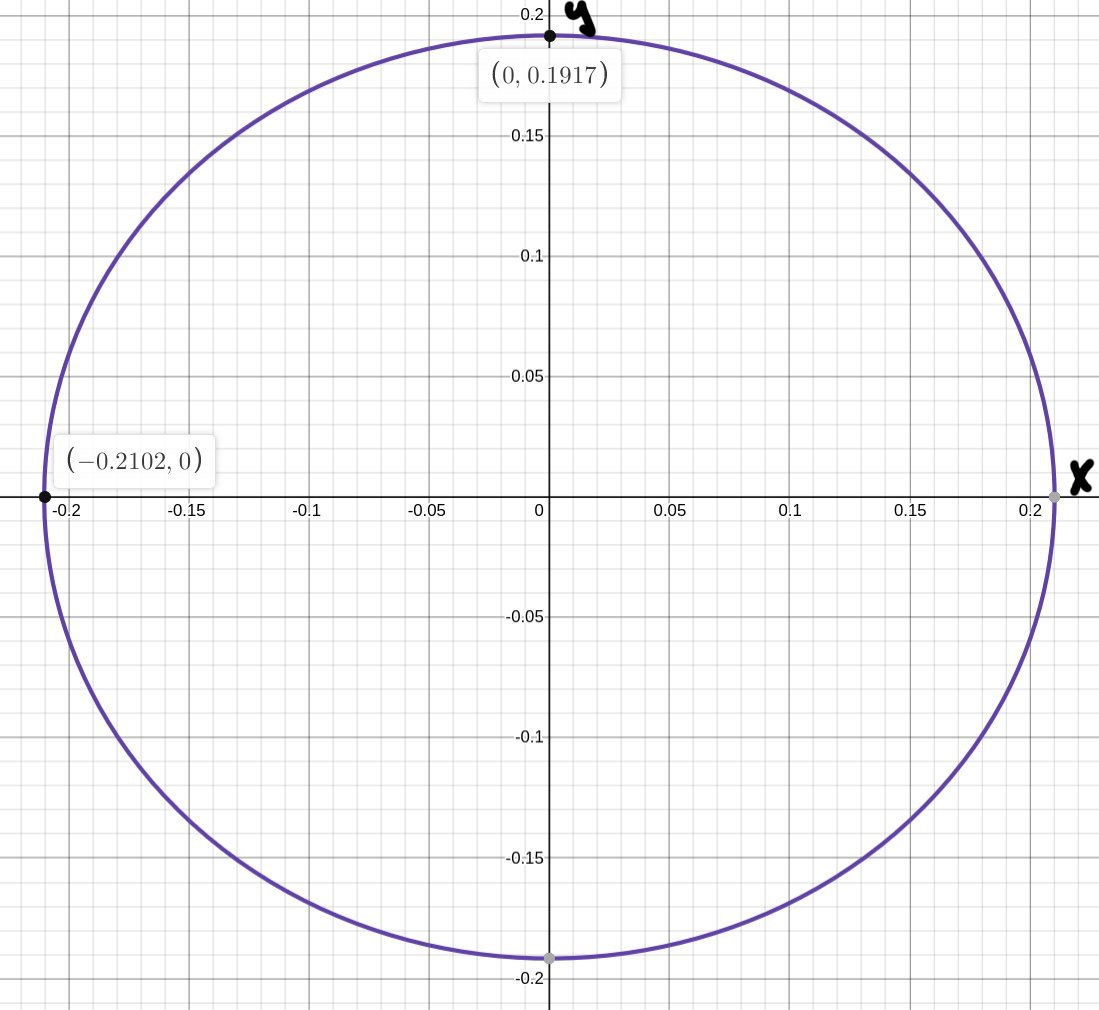
\includegraphics[width=1.13\linewidth]{pictures/graf1.png}
  \caption{xOy}
  \label{graf1}
\end{subfigure}%
\begin{subfigure}{.5\textwidth}
  \centering
  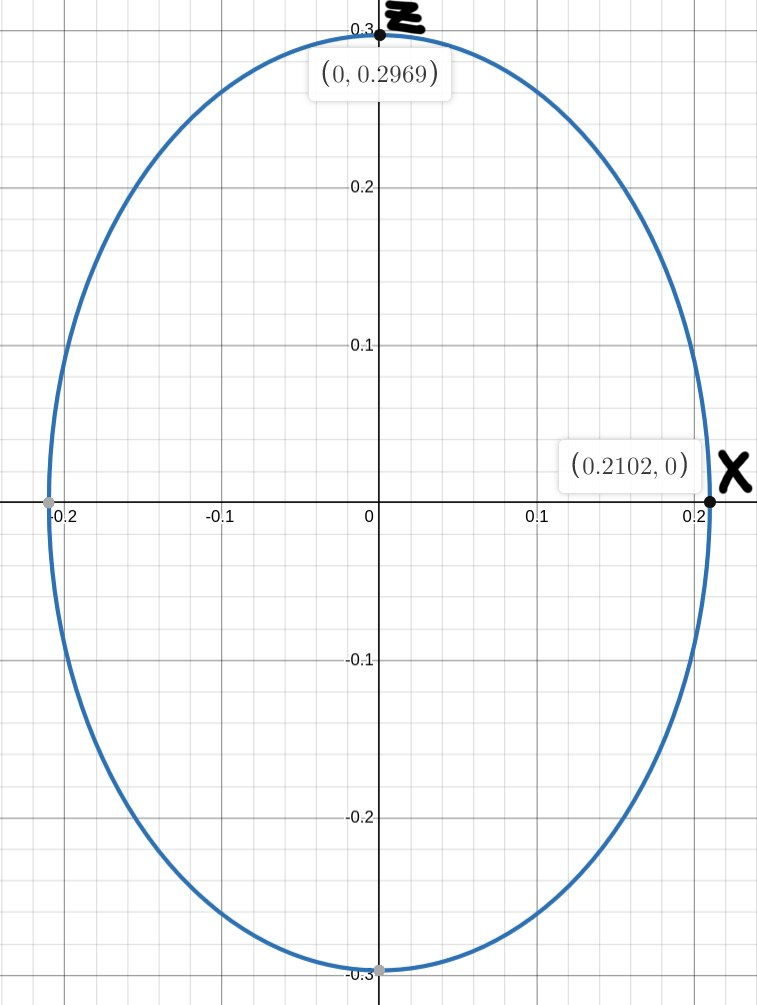
\includegraphics[width=0.8\linewidth]{pictures/graf2.png}
  \caption{xOz}
  \label{graf2}
\end{subfigure}
\label{fig:test}
\caption{Сечения эллипсоида инерции главными плоскостями}
\end{figure}

Из графика можно найти отношения эллипсоидов инерций:

$I_x / I_y \approx 0,831$

$I_x / I_z \approx 1,994$

Сравним с теоретическими значениями:

$I_x / I_y \approx 0,769$

$I_x / I_z \approx 2,004$

Значения совпали с неплохой точностью

\section{Вывод}

В результате опыта мы проверили симметрию параллелипипеда, а также эксперементально проверили уравнения (5) - (8), эксперементально нашли отношения моментов импульсов основных осей, которые с хорошей точностью совпали с теоретическими значениями.
